\documentclass[a4paper]{article}

\usepackage{libertine}
\usepackage{libertinust1math}
\usepackage{graphicx}
\usepackage{enumerate}

\usepackage{geometry}
\geometry{
  a4paper,
  left=2cm,
  right=2cm
}

\newcommand\dr{\mathrm}


\begin{document}

\begin{center}
  {\Large\textbf{Semantică distribuțională \\
      pentru analiza poeziilor}}

  \textsc{Adrian Manea, 510 SLA}
\end{center}

\section*{Ideea}

\indent\indent Lucrarea prezintă aspecte introductive de
\emph{semantică distribuțională} (SD), aplicate în studiul
poeziilor scrise în limba engleză.

După o introducere teoretică privitoare la subiectul și unele dintre metodele
utilizate în SD, prezentăm ca aplicație studiul coerenței subiectelor în
poezia engleză modernă și contemporană.

%%%%%%%%%%%%%%%%%%%%%%%%%%%%%%%%%%%%%%%%%%%%%%%%%%%%%%%%%%%%%%%%%%%%%%
\section*{Subiectul și metodele SD}

Această ramură a lingvisticii se bazează e \emph{ipoteza distribuțională},
formulată în anii '50, care afirmă că similaritatea semantică rezultă în
similarități ale unor distribuții statistice. Abordarea este, însă,
\emph{invers}: se pornește de la corpusuri de text și se induc reprezentări
semantice pe baza distribuțiilor observate.

\emph{Intuitiv:} ,,Sensul unui cuvînt este utilizarea lui în limbaj``
(L.\ Wittgenstein, 1922). În multe situații, putem ghici sensul unui cuvînt
din contextele în care acesta este folosit.

\emph{Modelul matematic:} spațiile vectoriale, numite în acest caz special,
\emph{spații semantice}.

\emph{Metoda}, într-o prezentare simplificată, se bazează pe ambiguitatea
termenului de ,,context``. Astfel, se stabilește un cuvînt-cheie căruia
se caută semantica și o fereastră de conținut, care în varianta cea mai
simplă înseamnă un interval centrat în cuvîntul-cheie, de o lungime
prestabilită, preluat din textul studiat. De obicei, se aplică rafinări
suplimentare contextului, e.g.\ ignorarea prepozițiilor, a punctuației sau
chiar concentrarea pe părțile de vorbire asociate, de obicei, cuvîntului-cheie
(e.g.\ dacă se studiază un substantiv, se poate acorda atenție suplimentară
adjectivelor și verbelor).

Se parcurg toate ferestrele de conținut de această formă și se înregistrează
cele mai numeroase co-ocurențe de cuvinte, asociate cuvîntului-cheie.
Rezultatele se stochează într-un vector asociat cuvîntului respectiv. Exemplu:
dacă corpusul studiat este \emph{Encyclopedia Britannica}, iar cuvîntul-țintă
este \emph{coleopter}, putem obține un vector de co-ocurențe de forma:
\[
  v = \begin{pmatrix}
    5221 & 4431 & 3111 & 2104 & 987 & 511 & 251 & 41
  \end{pmatrix},
\]
asociate cuvintelor, respectiv, \emph{mare, aripă, larvă, copac, floare, %
  cîmpie, cald, roșu}. Putem decide să ignorăm primul cuvînt, deoarece este
unul comun, care apare în preajma prea multor cuvinte pentru a fi decisiv
în ce privește sensul. La fel, ultimul cuvînt, care nu doar că ar putea fi
irelevant pentru semantica cuvîntului-țintă, dar are și un număr de apariții
comparativ mult mai mic față de celelalte. Însă celelalte sînt relevante
și ne dau de înțeles că ar putea fi vorba despre o insectă.

În exemplul de mai sus, spunem că folosim un spațiu vectorial cu un număr de
dimensiuni egal cu numărul de co-ocurențe asociate cuvîntului-cheie. Putem fie
să folosim toate cele 8 dimensiuni în cazul de mai sus, sau să păstrăm doar 6,
după o filtrare a celor relevante.

Ulterior, se pot aplica filtrări suplimentare, care pot avea diverse roluri care
să facă mai relevante cifrele calculate. În plus, una dintre cele mai importante
transformări ulterioare este calculul \emph{coeficientului de similaritate} între
doi vectori corespunzători la două cuvinte. Acesta se calculează ca fiind
cosinusul unghiului dintre vectorii asociați celor două cuvinte, folosind
produsul scalar euclidian.

%%%%%%%%%%%%%%%%%%%%%%%%%%%%%%%%%%%%%%%%%%%%%%%%%%%%%%%%%%%%%%%%%%%%%%

\section*{Aplicație: Coerența în poezia modernă și contemporană}

Punctul de pornire a acestei aplicații este critica adusă poeziei, conform
căreia acest tip de scriere nu are o semantică, întrucît cuvintele sînt folosite
cu sensuri mult diferite față de sensurile de dicționar. De aceea, dacă se
încearcă analiza \emph{coerenței subiectelor}, adică extragerea cuvintelor
care arată despre ce este vorba în poezia analizată, mult prea rar se constată
o coerență, adică se găsesc cuvinte care aparțin aceleiași familii lexicale.
De exemplu, o mulțime de subiecte de forma $ \{ $ scaun, masă, birou,
echipă $ \} $ are o coerență mai mare decît $ \{ $ scaun,
rece, elefant, nor $ \} $.

Se definește \emph{coerența unei mulțimi de cuvinte}
$ W = \{ w_i \mid 1 \leq i \leq n \} $
prin:
\[
  \overline{S}(W) = \overline{ \{ \dr{Sim}(w_i, w_j) \mid 1 \leq i < j \leq n \} },
\]
unde bara superioară notează media, iar $ \dr{Sim} $ reprezintă similaritatea,
calculată cu ajutorul cosinusului:
\[
  \dr{Sim}(A, B) = \dfrac{\sum A_i \cdot B_i}{\sqrt{\sum A_i^2 \cdot B_i^2}},
\]
iar mărimea ferestrei de conținut (mai precis, dimensiunea spațiului semantic)
este $ n = 2000 $, număr care s-a dovedit relevant și în alte studii.

În experiment, au fost alese 8 texte, dintre care 6 sînt poezii moderne și
contemporane, iar 2 au fost de control: un text generat aleatoriu și un text
de pe Wikipedia. Textelor s-au atribuit scoruri de dificultate a înțelegerii,
iar rezultatul studiului coerenței este cel din figura \ref{fig:coe}.

\begin{figure}[!htb]
  \centering
  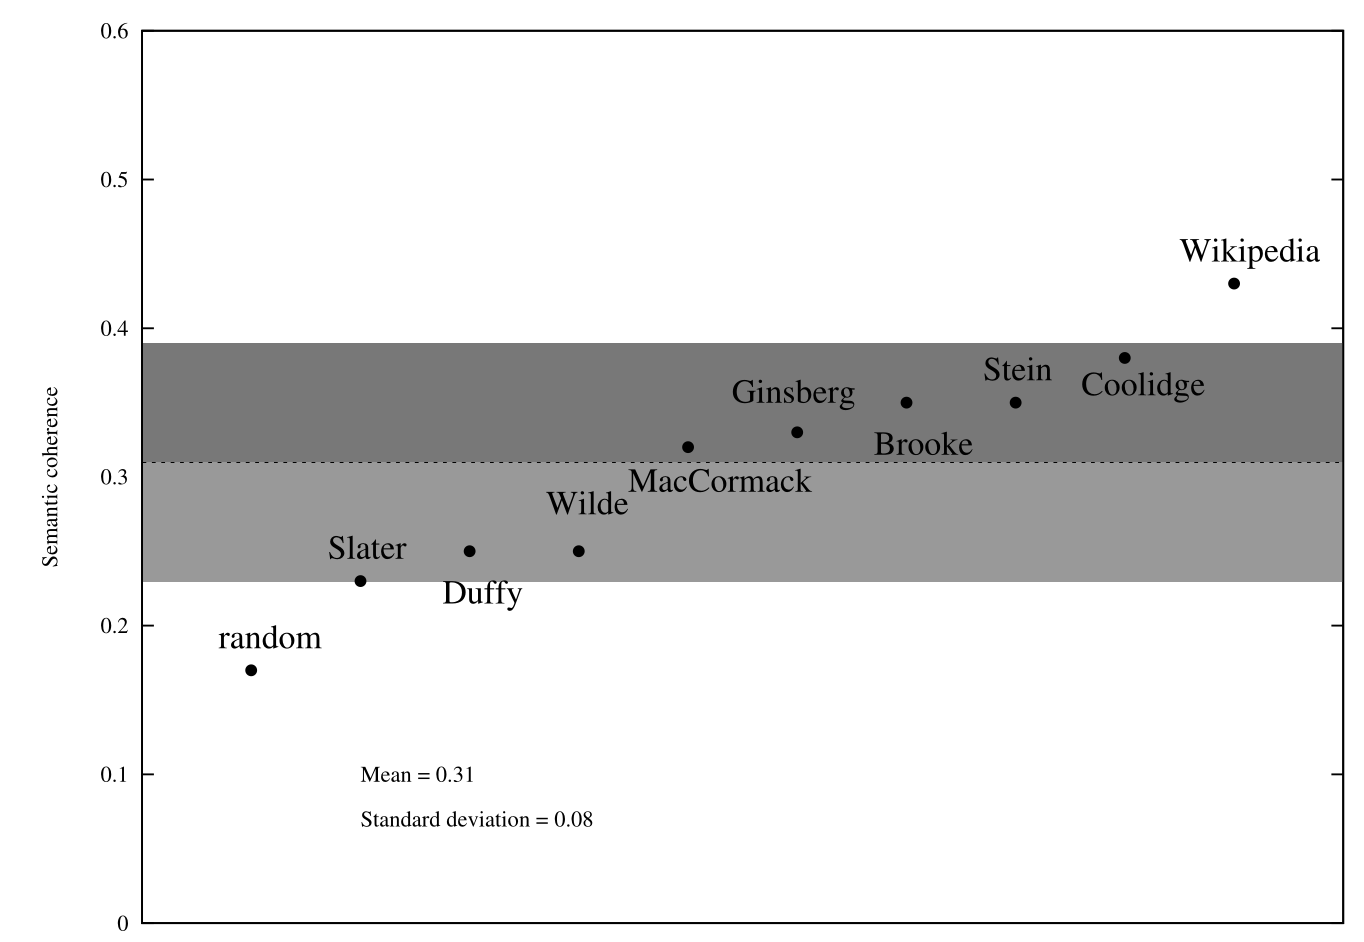
\includegraphics[scale=0.2]{img/coherence1.png}
  \caption{Coerența subiectelor din poezii moderne și contemporane}
  \label{fig:coe}
\end{figure}

Concluziile studiului au fost că nu se evidențiază discrepanța pe care unii
critici au remarcat-o între coerența subiectelor din limbajul comun
și cea a limbajului poetic. În plus, putem constata din grafic faptul că
poeziile se situează undeva la mijloc între un text aleatoriu (deloc coerent)
și unul științfic (cu coerența maximă). Și mai mult decît atît, dificultatea
de înțelegere a textului nu este legată de coerența subiectelor. Astfel,
textul lui MacCormarck a fost apreciat drept cel mai greu de înțeles
(după cel generat aleatoriu), dar observăm că el are un scor mediu de coerență.
Pe de altă parte, textul lui Stein a fost apreciat ca fiind mediu de înțeles,
iar coerența sa este foarte mare.

Pentru o și mai bună claritate, s-au adăugat texte suplimentare de control,
unele generate aleatoriu și unele factuale (științifice). Tendința de a se situa
la mijloc se vede mai accentuat, conform figurii \ref{fig:coe2}.

\begin{figure}[!htb]
  \centering
  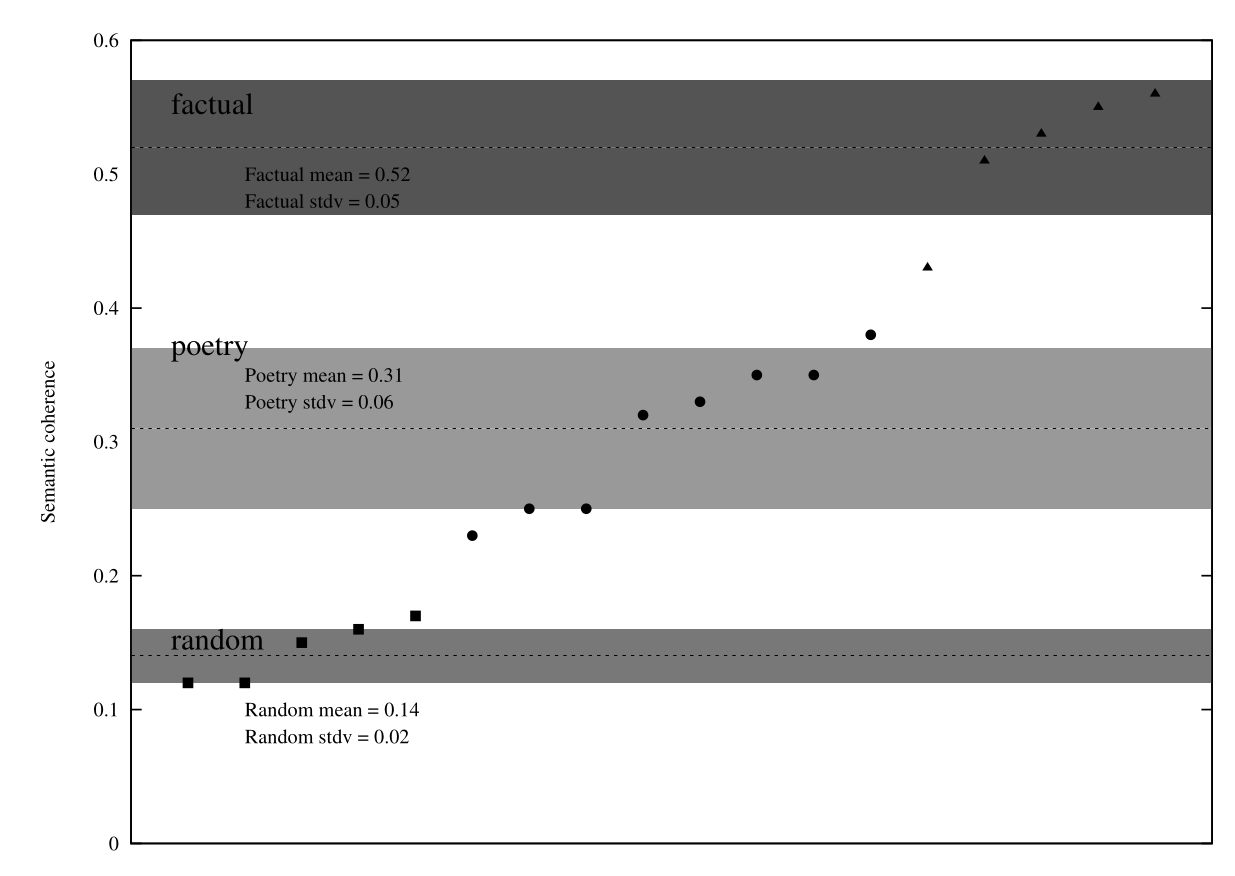
\includegraphics[scale=0.2]{img/coherence2.png}
  \caption{Coerența poeziilor, cu texte de control suplimentare}
  \label{fig:coe2}
\end{figure}

\newpage

\section*{Bibliografie selectivă}

\begin{enumerate}[(1)]
\item Erk, K. -- \emph{Vector space models of word meaning and phrase meaning: A survey},
Language and Linguistics Compass, 2012;
\item Herbelot, A. -- \emph{The Semantics of Poetry: A Distributional Reading},
  Digit.\ Scholarsh.\ Humanit., 2015;
\item Turney, P., Pantel, P. -- \emph{From frequency to meaning: Vector space %
  models of semantics}, J.\ Artif.\ Intell.\ Res., 2010.
\end{enumerate}


\end{document}
